La responsabilità di gestione del progetto è attribuita al \textit{Responsabile di Progetto}. \\
Utilizzando tutti gli strumenti a disposizione il \textit{Responsabile di Progetto} avrà il compito di:
\begin{itemize}
	\item Pianificare le attività;
	\item Gestire le risorse;
	\item Analizzare e prevenire i rischi.
\end{itemize}

\subsubsection{Pianificazione}

\paragraph{Pianificazione delle attività}
Per pianificare le varie attività da svolgere il \textit{Responsabile di Progetto} dovrà utilizzare \gls{GanttProject} per realizzare i diagrammi di \gls{Gantt}.

\paragraph{Coordinazione e gestione delle risorse}
Per gestire le risorse durante lo sviluppo del progetto, il \textit{Responsabile di Progetto} dovrà pianificare la quantità di ore che ogni risorsa dovrà dedicare a ciascuna attività.\\
Si è deciso di utilizzare il servizio di gestione dei \gls{task} e creazione di \gls{milestone} offerto da \gls{GitHub} spiegato nella sezione \ref{ticket}. Questo permette di accentrare le informazioni in un solo ambiente.
	\subparagraph{Rotazione dei ruoli:}
	Ogni membro del gruppo dovrà ricoprire tutti i ruoli definiti nel \textit{Piano di Progetto v3.0.0}. Il \textit{Responsabile di Progetto} avrà il compito di pianificare l'impiego delle risorse in modo equo e in modo che ogni risorsa ricopra tutti i ruoli. 
	Si deve controllare attentamente che non vi siano conflitti di interesse specialmente nelle attività di approvazione e verifica. Per garantire che la rotazione dei ruoli non provochi conflitti è necessario che le attività vengano pianificate con attenzione e che i membri interessati rispettino ruoli e compiti loro assegnati. Spetterà al \textit{Verificatore} controllare che tutte le condizioni sopra indicate vengano rispettate. Se il \textit{Verificatore} troverà delle incongruenze con quanto menzionato sopra avrà il compito di avvisare il \textit{Responsabile di Progetto} che dovrà risolvere la questione.\\
	Ogni componente del gruppo potrà consultare, in qualsiasi momento, i diagrammi di \gls{Gantt} che descrivono la gestione delle risorse e dei ruoli, in maniera tale che ognuno potrà sempre essere consapevole del ruolo ricoperto dagli altri componenti.

\paragraph{Analisi e prevenzione dei rischi}
Durante l'avanzamento del progetto, il \textit{Responsabile di Progetto} deve monitorare costantemente il verificarsi dei rischi descritti nel \textit{Piano di Progetto v3.0.0}. La valutazione dei rischi deve essere aggiornata al mutare delle situazioni di pericolo, in occasione di significative modifiche al processo produttivo oppure all'introduzione di nuove tecnologie. Una volta completata la valutazione dei rischi si dovrà redigere una relazione scritta, modificando e aggiornando il \textit{Piano di Progetto}, contenente le misure di prevenzione previste e il loro programma di attuazione.

\newpage
\subsubsection{Esecuzione e controllo}
		\paragraph{Riunioni}
		Il \textit{Responsabile di Progetto} ha il compito di indire le riunioni, sia interne che esterne. Per ogni riunione sarà necessario specificare data, ora, luogo, e l'ordine del giorno. Le informazioni sulla riunione dovranno essere rese disponibili con almeno quattro giorni di anticipo.
		\subparagraph{Interne:}
		Sarà il \textit{Responsabile di Progetto} a convocare i componenti del gruppo alle riunioni generali. Tutti i membri del team dovranno partecipare fisicamente o in videochiamata. Le riunioni avranno una frequenza almeno quindicinale. Ogni componente del gruppo è tenuto a leggere la posta elettronica ed a rispondere ad eventuali richieste di riunioni interne. \\
		Il \textit{Responsabile di Progetto} può anticipare o posticipare una riunione in base alla disponibilità data dai componenti del gruppo. È possibile richiedere una riunione generale da parte di un qualsiasi componente del gruppo. La richiesta verrà inoltrata al \textit{Responsabile di Progetto} che potrà decidere se accoglierla o rifiutarla.\\
		Inoltre, è possibile ed auspicabile che siano necessarie riunioni tra specifici membri del gruppo, ad esempio: in fase di analisi può essere utile che solo gli \textit{Analisti} si incontrino tra di loro. I componenti che non hanno presieduto la riunione saranno comunque informati sui contenuti e sulle decisioni prese tramite invio di una email alla mailing list o pubblicazione di un \gls{verbale} sul \gls{repository} nel caso siano state prese decisioni importanti.
		\subparagraph{Esterne:}
		Sarà il \textit{Responsabile di Progetto} a fissare le riunioni esterne con i Proponenti e/o i Committenti utilizzando la casella di posta elettronica creata appositamente. Prima di contattare le parti esterne, il \textit{Responsabile di Progetto} dovrà verificare la presenza dei membri interni del gruppo. \\
		In caso di risposta positiva si provvederà a contattare i Proponenti e/o i Committenti per fissare la data dell'incontro.
		È compito del \textit{Responsabile di Progetto} di redigere il \gls{verbale} dell'incontro avvenuto.
		
		\paragraph{Comunicazioni}
			\subparagraph{Comunicazioni interne:}
			Le comunicazioni interne verranno eseguite attraverso la mailing list: \url{dazzleworksgroup@gmail.com}. \\ 
			Quando un membro del gruppo vuole inviare una email a tutti i componenti, deve inviare il messaggio dalla sua casella di posta elettronica personale verso l'indirizzo \url{dazzleworksgroup@gmail.com}, dalla quale un inoltro automatico provvederà a mandare l'email agli altri indirizzi di posta elettronica personali dei componenti del gruppo, tenendo traccia di tutte le comunicazioni.\\ 
			I membri sono tenuti a prestare attenzione al numero di messaggi diffusi. È sempre importante non arrivare a una sovraesposizione del pubblico interno, in quanto si creerebbe solo senso di smarrimento e confusione. Questo non esclude che uno stesso messaggio non sia proposto su più mezzi di informazione, azione spesso necessaria, ma questo presuppone un intervento ponderato e non casuale.\\
			Con lo scopo di facilitare la comunicazione tra i membri del gruppo vengono utilizzati strumenti di messaggistica istantanea e videochiamata come \gls{Skype} e \gls{Google Hangouts}.
			È necessario redigere un \gls{verbale} nel caso in cui siano state prese decisioni o siano emersi dettagli inerenti allo sviluppo del progetto. 
			\subparagraph{Comunicazioni esterne:}
			Per le comunicazioni esterne è stato creato un indirizzo di posta elettronica:
			\begin{center}
				\url{dazzleworksgroup@gmail.com}
			\end{center}
			Tale indirizzo deve essere l'unico canale di comunicazione verso l'esterno. Sarà solo il \textit{Responsabile di Progetto} ad utilizzare l'indirizzo di posta per intrattenere le corrispondenze con i Proponenti e i Committenti. È compito del \textit{Responsabile di Progetto} informare i membri del gruppo delle discussioni avvenute ed eventualmente inoltrare i messaggi alla mailing list.
			
		\paragraph{Composizione email}
			In questo paragrafo viene descritta la forma che deve avere una email sia per comunicazione interna che esterna.
			\subparagraph{Mittente:}
			\begin{itemize}
				\item \textbf{Interno:} indirizzo personale di chi scrive il messaggio;
				\item \textbf{Esterno:} l'unico indirizzo utilizzabile per comunicare verso l'esterno è \url{dazzleworksgroup@gmail.com} e deve essere usato esclusivamente dal \textit{Responsabile di Progetto}.
			\end{itemize}
			\subparagraph{Destinatario:}
			\begin{itemize}
				\item \textbf{Esterno:} l'indirizzo del destinatario può avere variazioni a seconda che si voglia comunicare con il Prof. Tullio Vardanega, il Prof. Riccardo Cardin o con i Proponenti del progetto;
				\item \textbf{Interno:} l'unico indirizzo utilizzabile è \url{dazzleworksgroup@gmail.com}.
			\end{itemize}
			Le uniche eccezioni permesse sono:
			\begin{itemize}
				\item \textbf{Proposte all'\textit{Amministratore di Progetto}:} per eventuali proposte di cambiamento delle norme da parte di un membro del gruppo, quest'ultimo dovrà contattarlo al suo indirizzo di posta elettronica personale;
				\item \textbf{Comunicazione ristretta tra alcuni membri del gruppo:} in questi casi i membri del gruppo utilizzeranno i loro indirizzi personali.
			\end{itemize}
			
			\subparagraph{Oggetto:}
			L'oggetto deve sintetizzare il contenuto della email. Deve essere chiaro, breve e possibilmente univoco in modo da riconoscerlo da quelli precedenti.\\
			Nel caso si debba mandare un messaggio alla mailing list è obbligatorio aggiungere "Group:" all'inizio dell'oggetto.
			\subparagraph{Corpo:}
			Il corpo del messaggio deve essere chiaro, diretto e avere tutte le informazioni necessarie per permettere a tutti i destinatari di capire correttamente l'argomento trattato. Per riferirsi ad alcuni componenti del gruppo o ruoli di progetto si dovrà usare la seguente sintassi: "\textbf{Cognome Nome}" o "\textbf{Nome Ruolo}". Alla fine del corpo del messaggio, il mittente dovrà sempre firmarsi con il suo nome, cognome e ruolo all'interno del gruppo.
			\subparagraph{Allegati:}
			Viene consentito l'uso di allegati che deve essere limitato solo al caso in cui essi siano realmente necessari. È buona norma presentare gli allegati scrivendo alcune righe di spiegazione. Prestare attenzione al formato(preferibilmente PDF) del documento che si sta inviando. 
			
\newpage
		\paragraph{Gestione ticket e milestone} \label{ticket}
		Per la gestione dei ticket e la creazione di milestone viene utilizzato il servizio di ticketing offerto da GitHub. 
		\subparagraph{Creazione e gestione dei ticket:} 
		
		I \gls{ticket} vengono creati e gestiti quasi tutti dal \textit{Responsabile di Progetto}.
		Qualora il \textit{Verificatore} trovasse imprecisioni o errori durante la verifica, avrà la possibilità di creare dei \gls{ticket} per segnalare suddetti errori.
		Ogni \gls{ticket} può essere assegnato ad uno o più membri del gruppo a seconda della complessità del lavoro e della disponibilità dei membri del gruppo.
		Per creare un nuovo \gls{ticket} bisogna:
		
		\begin{itemize}
			\item Posizionarsi alla voce Issue;
			\item Premere "New issue";
			\item Compilare i campi richiesti:
			\begin{itemize}
				\item \textbf{Titolo e commenti:} titolo descrittivo con una descrizione del nuovo \gls{ticket};
				\item \textbf{Labels:} dovranno avere due caratteristiche fondamentali e cioè la tipologia di \gls{ticket} assegnato(modifica, verifica, richiesta approvazione) e la priorità assegnata(alta, media, bassa);
				\item \textbf{\gls{Milestone}:} la \gls{milestone} a cui è associato il \gls{ticket};
				\item \textbf{Assignee:} a chi viene assegnato il \gls{ticket}.
			\end{itemize}
		\end{itemize}
		\begin{figure}[h]
			\centering
			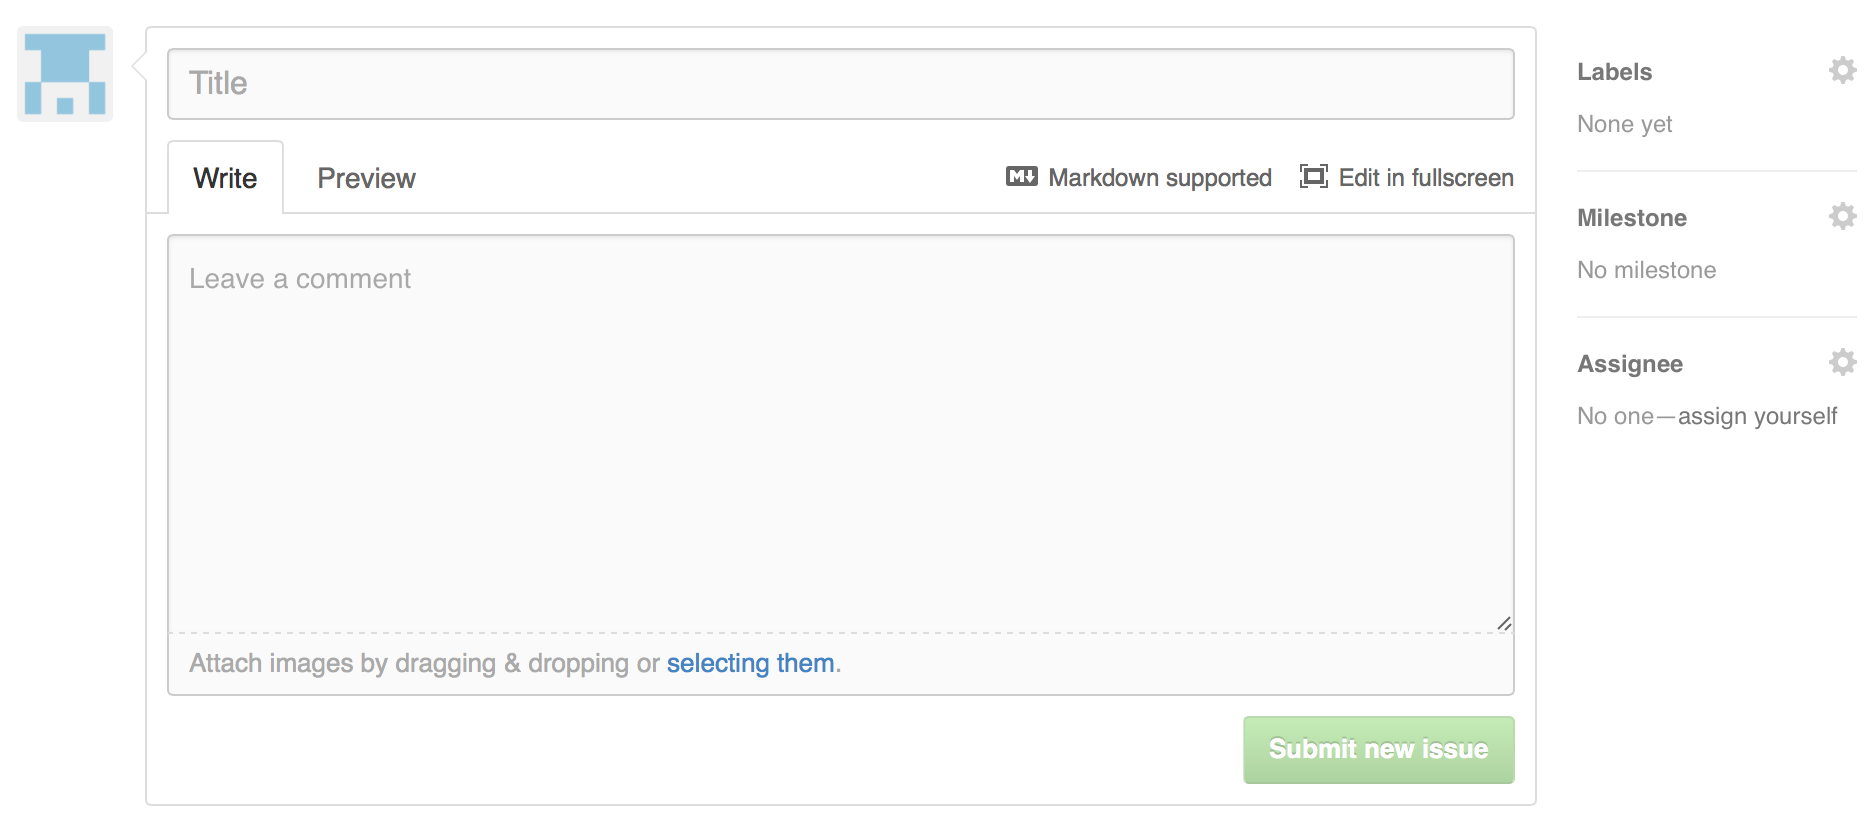
\includegraphics[width=1\linewidth]{img/ticket}
			\caption[Creazione ticket]{Creazione ticket}
			\label{fig:ticket}
		\end{figure}
		
		\newpage
		\subparagraph{Creazione delle milestone:}
		
		Il \textit{Responsabile di Progetto} ha il compito della creazione di una \gls{milestone} in occasione di ogni revisione al quale il gruppo \GRUPPO\ ha intenzione di partecipare, più altre \gls{milestone} qualora il \textit{Responsabile di Progetto} lo ritenga necessario.
		
		Per creare una nuova \gls{milestone} bisogna:
		
		\begin{itemize}
			\item Posizionarsi alla voce \gls{Milestone};
			\item Premere "New \gls{milestone}";
			\item Compilare i campi richiesti:
			\begin{itemize}
				\item \textbf{Titolo;}
				\item \textbf{Descrizione;}
				\item \textbf{Data.}
			\end{itemize}
		\end{itemize}
		\begin{figure}[h]
			\centering
			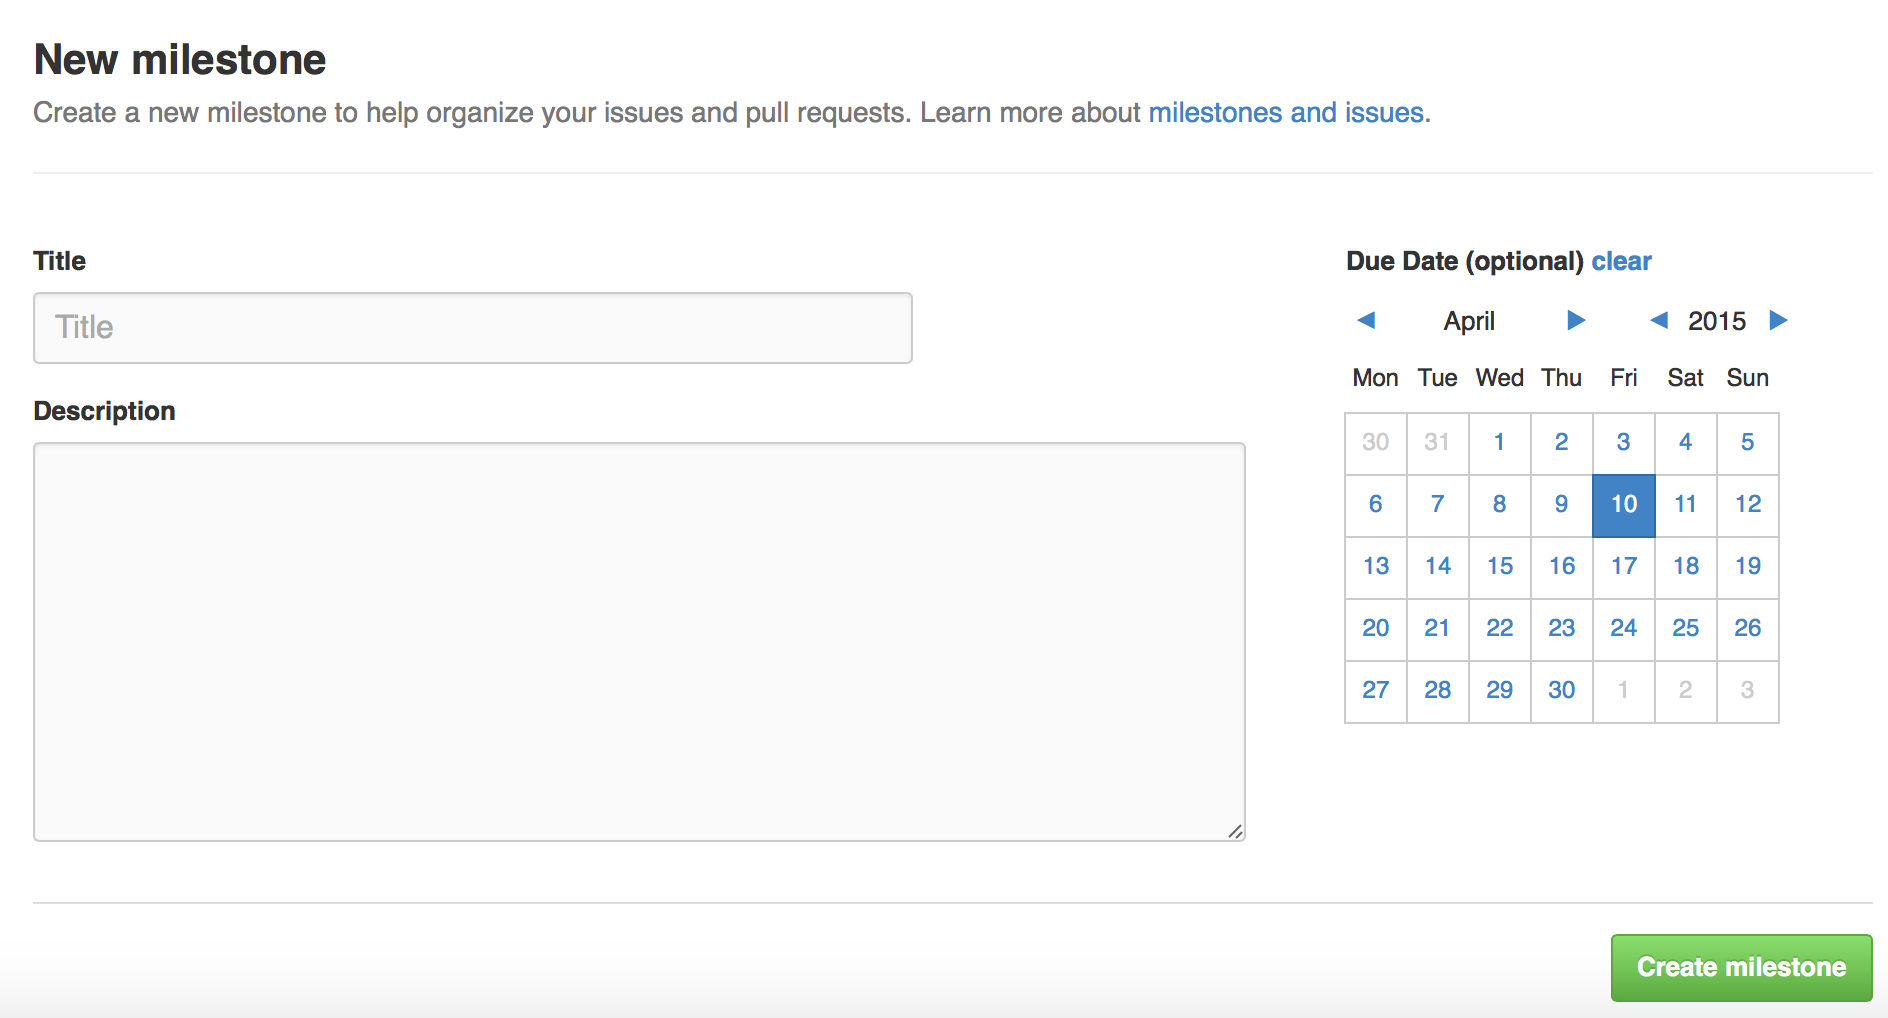
\includegraphics[width=1\linewidth]{img/milestone}
			\caption[Creazione milestone]{Creazione milestone}
			\label{fig:milestone}
		\end{figure}
		
		\subparagraph{Esecuzione dei compiti:}
		
		Ogni membro del gruppo è tenuto a visionare regolarmente la presenza di \gls{ticket} a lui assegnati e segnalarne la presa in consegna.
		Una volta che un membro porta a termine un \gls{ticket} deve modificarne lo stato per segnalare il termine del lavoro.
		Se un \gls{ticket} non ha avuto i risultati attesi il \textit{Responsabile di Progetto} può riaprirlo ed eventualmente assegnare altri membri al lavoro.
		
		\subparagraph{Chiusura della milestone:}
		
		Una volta raggiunta la scadenza il \textit{Responsabile di Progetto} deve chiudere la \gls{milestone} ed eventualmente aprirne un'altra per poi ricominciare tutto il protocollo da capo.

\newpage
\subsubsection{Norme generali}
	\paragraph{Ambiente di sviluppo}
	Secondo il decreto legislativo n.81, ogni 120(centoventi) minuti passati in maniera continuativa davanti al computer ogni membro deve fare almeno quindici minuti interruzione.\footnote{\url{http://www.pmi.it/impresa/normativa/news/51788/dipendenti-al-pc-obblighi-di-legge-per-i-datori-di-lavoro.html}}

	\paragraph{Ruoli di Progetto}
	Lo sviluppo prevede la collaborazione di individui a cui verranno assegnati ruoli diversi. Tali ruoli rappresentano figure aziendali specializzate, indispensabili per il buon esito del progetto.\\
Di seguito i diversi ruoli di progetto con le relative responsabilità e modalità operative.
\subsection{Responsabile di Progetto}
Il \textit{Responsabile di Progetto} rappresenta il progetto, in quanto accentra su di sé la responsabilità di scelta e approvazione, ed il gruppo, poiché presenta al committente i risultati del lavoro svolto.
Detiene il potere decisionale, quindi la responsabilità in merito a:
\begin{itemize}
	\item Pianificazione, coordinamento e controllo delle attività;
	\item Gestione e controllo delle risorse;
	\item Analisi e gestione dei rischi;
	\item Approvazione dei documenti;
	\item Approvazione dell'offerta economica.
\end{itemize}
Di conseguenza, ha il compito:
\begin{itemize}
	\item Assicurarsi che le attività di verifica e validazione vengano svolte sistematicamente seguendo le \textit{Norme di Progetto v2.0.0};
	\item Garantire che vengano rispettati i ruoli e le competenze assegnate nel \textit{Piano di Progetto};
	\item Garantire che non vi siano conflitti tra \textit{Verificatori} e \textit{Redattori};
	\item Gestire la creazione e l'assegnazione dei \gls{ticket} ad ogni membro del gruppo.
\end{itemize}
\subsection{Ammministratore}
L'\textit{Amministratore di Progetto} è il responsabile dell'efficienza e del rendimento nell'ambiente di lavoro. Le mansioni che gli competono sono le seguenti:
\begin{itemize}
	\item Agevolare le attività richieste dalle \textit{Norme di Progetto v2.0.0};
	\item Ricercare e rendere operativi tutti gli strumenti necessari all'automatizzazione del maggior numero di compiti;
	\item Fornire procedure e strumenti per il controllo e la segnalazione del controllo qualità;
	\item Gestire l'archiviazione e il \gls{versionamento} della documentazione;
	\item Controllare le versioni dei prodotti e gestire le loro configurazioni.
\end{itemize}
Redige le \textit{Norme di Progetto}, dove spiega e norma l'utilizzo degli strumenti, e redige la sezione del \textit{Piano di Qualifica} dove vengono descritti strumenti e metodi di verifica.
\subsection{Analista}
L'\textit{Analista} è il responsabile delle attività di analisi. Le mansioni che gli competono sono:
\begin{itemize}
	\item Comprendere appieno la natura e la complessità del problema;
	\item Produrre una \textit{specifica di progetto} motivata in ogni suo punto e comprensibile a tutti gli interessati.
\end{itemize}
Redige lo \textit{Studio di Fattibilità}, l'\textit{Analisi dei Requisiti} e partecipa alla redazione del \textit{Piano di Qualifica} in quanto conosce l'ambito di progetto.

\subsection{Progettista}
Il \textit{Progettista} è il responsabile delle attività di progettazione. La mansioni che gli competono sono:
\begin{itemize}
	\item Produrre una soluzione comprensibile, attuabile e motivata;
	\item Effettuare scelte su aspetti progettuali che applichino al prodotto soluzioni note ed ottimizzate;
	\item Effettuare scelte su aspetti progettuali e tecnologici che rendano il prodotto facilmente manutenibile.
\end{itemize}
Redige la \textit{Specifica Tecnica}, la \textit{Definizione di Prodotto} e le sezioni relative alle metriche di verifica della programmazione del \textit{Piano di Qualifica}.

\subsection{Verificatore}
Il \textit{Verificatore} è il responsabile delle attività di verifica. Le mansioni che gli competono sono:
\begin{itemize}
	\item Garantire che l'attuazione delle attività sia conforme alle norme stabilite;
	\item Verificare che non siano stati introdotti errori lungo il percorso;
	\item Controllare la conformità di ogni stadio del ciclo di vita del prodotto.
\end{itemize}
Redige la sezione del \textit{Piano di Qualifica} che illustra l'esito e la completezza delle verifiche
e delle prove effettuate.

\subsection{Programmatore}
Il \textit{Programmatore} è responsabile delle attività di codifica e delle componenti di ausilio necessarie per l'esecuzione delle prove di verifica e validazione. Le mansioni che gli competono sono:
\begin{itemize}
	\item Implementare in maniera rigorosa le soluzioni descritte dal \textit{Progettista};
	\item Scrivere codice che sia documentato, versionato, manutenibile e che rispetti le metriche stabilite per la scrittura del codice;
	\item Implementare i test sul codice prodotto, necessari per le prove di verifica e validazione.
\end{itemize}
Redige il \textit{Manuale Utente}.

\subsection{Rotazione dei ruoli}
Ogni membro del gruppo dovrà ricoprire tutti i ruoli definiti nel \textit{Piano di Progetto v2.0.0}. Il \textit{Responsabile di Progetto} avrà il compito di pianificare l'impiego delle risorse in modo equo e in modo che ogni risorsa ricopra tutti i ruoli. 
Si deve controllare attentamente che non vi siano conflitti di interesse specialmente nelle attività di approvazione e verifica. Per garantire che la rotazione dei ruoli non provochi conflitti è necessario che le attività vengano pianificate con attenzione e che i membri interessati rispettino ruoli e compiti loro assegnati. Spetterà al \textit{Verificatore} controllare che tutte le condizioni sopra indicate vengano rispettate. Se il \textit{Verificatore} troverà delle incongruenze con quanto menzionato sopra avrà il compito di avvisare il \textit{Responsabile di Progetto} che dovrà risolvere la questione.\\
Ogni componente del gruppo potrà consultare, in qualsiasi momento, i diagrammi di \gls{Gantt} che descrivono la gestione delle risorse e dei ruoli, in maniera tale che ognuno potrà sempre essere consapevole del ruolo ricoperto dagli altri componenti.


	
\newpage
	\paragraph{Struttura del repository} \label{repository}
	Per la gestione della documentazione e della codifica sono stati creati due \gls{repository}. Un \gls{repository} privato e, quindi, accessibile solo dai membri del gruppo \GRUPPO per la documentazione e un \gls{repository} pubblico per contenere il codice.\\
	Dopo l'ultima revisione il progetto verrà reso open-source.
	Per il \gls{repository} abbiamo scelto di usare il servizo \gls{GitHub}, il quale utilizza il sistema di \gls{versionamento} \gls{Git}.
	
	\subparagraph{Repository per la documentazione:}
	Tutta la documentazione si può trovare in un \gls{repository} disponibile al seguente indirizzo: \url{https://github.com/FabioRos/Premi}. \\
	Esso avrà questa struttura:
	\begin{itemize}
		\item \textbf{Interni:}
			\begin{itemize}
				\item \textbf{Studio di Fattibilità};
				\item \textbf{Norme di Progetto}.
			\end{itemize}
		\item \textbf{Esterni:}
			\begin{itemize}
				\item \textbf{Analisi dei Requisiti};
				\item \textbf{Piano di Progetto};
				\item \textbf{Piano di Qualifica};
				\item \textbf{Specifica Tecnica};
				\item \textbf{Definizione di Prodotto};
				\item \textbf{Glossario};
				\item \textbf{Lettera di Presentazione};
				\item \textbf{Verbali}.
			\end{itemize}
	\end{itemize}
	
	\subparagraph{Repository per il codice}
	Tutto il codice prodotto si può trovare in un \gls{repository} disponibile all'indirizzo: \url{https://github.com/DazzleWorks/Premi}.
	
\newpage
	\subparagraph{Norme sull'utilizzo del servizio:}
	È necessario eseguire le operazioni di sincronizzazione all'inizio e alla fine di ogni sessione di lavoro. \\
	In particolare ad ogni sessione di lavoro andranno eseguite le seguenti operazioni:
	\begin{itemize}
		\item \textbf{Pull}: scaricare la versione più aggiornata del progetto per poterci poi lavorare offline;
		\item \textbf{Add}: aggiungere i file ad uno specifico elenco generando una proposta di modifica;
		\item \textbf{Commit}: validare le proposte fatte in precedenza;
		\item \textbf{Push}: serve a pubblicare i risultati online, sulla piattaforma di sviluppo;
		\item \textbf{Merge}: permette di fondere un \gls{branch} con il \gls{repository} padre, così da implementare le modifiche apportate ai file e alle cartelle originarie.
	\end{itemize}
	\begin{figure}[h]
		\centering
		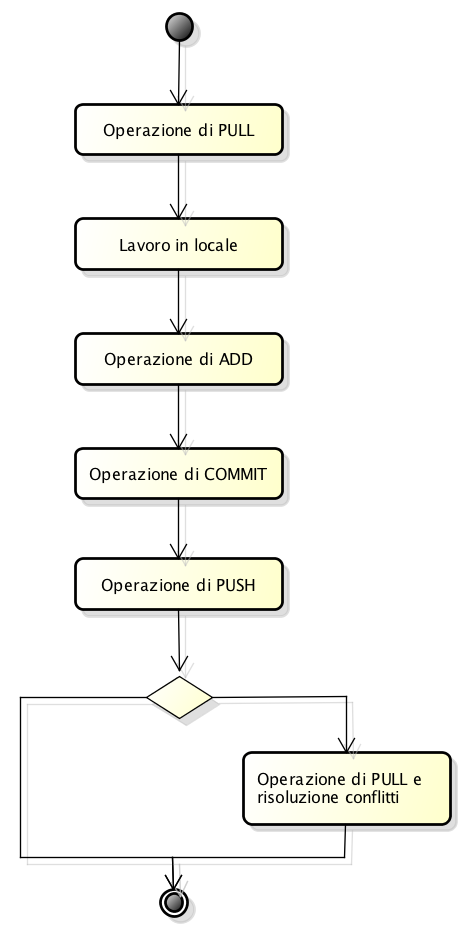
\includegraphics[width=0.5\linewidth]{img/proceduraRepository}
		\caption[Procedura per l'utilizzo del Repository]{Procedura per l'utilizzo del Repository}
		\label{fig:proceduraRepository}
	\end{figure}
	
	\noindent È vietato utilizzare "git add *" per evitare di includere file nascosti. Tutti i membri del gruppo dovono essere consapevoli dell'esatto contenuto dei file. Ogni commit deve essere corredato di un messaggio che descriva in modo \gls{conciso} il lavoro svolto.
				
\subsubsection{Strumenti}
	In questa sezione verrà illustrato l'ambiente di lavoro che sarà utilizzato durante lo sviluppo del progetto \PROGETTO.\\

\paragraph{Sistema operativo}

Il sistema operativo utilizzato è lasciato a discrezione di ogni membro del gruppo. Questa scelta è dovuta principalmente al fatto che il progetto dovrà supportare più piattaforme.
I membri del gruppo utilizzeranno i seguenti sistemi operativi:

\begin{itemize}
	\item \gls{Windows} 7 64 bit;
	\item \gls{Windows} 8.1;
	\item \gls{Ubuntu} 14.10;
	\item Mac OS 10.10.2.
\end{itemize}

\paragraph{Coordinamento}

Il coordinamento del gruppo avviene tramite:
\begin{itemize}
	\item \gls{Google Drive};
	\item \gls{Google Calendar};	
	\item \gls{Repository} \gls{Git}.
\end{itemize}

\subparagraph{Google Drive:}

Abbiamo scelto di utilizzare questo \gls{servizio cloud} per condividere tutti i documenti che non necessitano di \gls{versionamento} e vengono utilizzati frequentemente da parte dei membri del gruppo. 
È un servizio molto semplice e accessibile direttamente da \gls{browser} che permette di lavorare su documenti creati con \gls{Google Docs}.

\subparagraph{Google Calendar:}
\gls{Google Calendar} viene utilizzato per la gestione delle risorse umane e per tenere traccia degli eventi importanti. È stato creato un calendario condiviso con tutti i membri del gruppo in modo da conoscere le date in cui una persona è assente o non reperibile e le date rilevanti per il gruppo.\\
Inoltre è possibile modificare la gestione delle notifiche per un evento o più eventi in modo che venga inviata automaticamente una email a tutti i membri del gruppo. In questo caso il preavviso deve essere di almeno un giorno.

\subparagraph{Repository Git:}

Nonostante siano disponibili molti \gls{repository} (\gls{Git}, \gls{Mercurial}, \gls{SVN}) è stato scelto di utilizzare \gls{Git} in quanto il servizio soddisfa pienamente le necessità di \gls{hosting} e \gls{versionamento} necessarie per lo sviluppo di questo progetto, inoltre diversi membri del gruppo avevano già usato tale servizio. Esso permette di lavorare senza una connessione attiva a internet e da la possibilità di ignorare alcune estensioni specificate in un file chiamato .gitignore\footnote{File globale di \gls{Git} che contiene una lista di regole per ignorare i file.}.\\ Per i membri del gruppo che desiderano utilizzare un client, si consigliano i seguenti:
\begin{itemize}
	\item \textbf{SourceTree};
	\item \textbf{\gls{GitHub}};
\end{itemize}
Per maggiori dettagli sulle norme che riguardano l'utilizzo si rimanda alla sezione \ref{repository}.

\newpage
\paragraph{Ambiente documentale}

\subparagraph{Stesura documenti:}

Per la stesura dei documenti verrà utilizzato il \gls{linguaggio di markup} \LaTeX.
Come editor è consigliato TeXstudio\footnote{\url{http://texstudio.sourceforge.net}}, il quale è disponibile per tutti i principali sistemi operativi.

\subparagraph{Script:}

Per facilitare la stesura dei documenti sono stati creati alcuni script:

\begin{itemize}
	\item Generazione di tutti i documenti PDF: con il comando "make all" verranno generati tutti i PDF dei documenti contenuti nella directory corrente;
	%\item Controllo ortografico: con il comando make aspell verrà invocato il programma aspell su tutti i documenti della directory corrente;
	%\item Eliminazione file errati o vecchi: con il comando make clean verranno eliminatati i file generati da compilazioni vecchio o file non necessari della directory corrente;
	\item Evidenziare glossario: con il comando "java glossary" verrà eseguito uno script che selezionerà nei documenti della directory corrente le parole contenute nella versione più recente del glossario e le evidenzierà con il simbolo "\G".

\end{itemize}

\paragraph{Pianificazione delle attività}
Per pianificare le attività e la gestione del progetto e delle risorse umane si è scelto di usare \gls{GanttProject}\footnote{\url{http://www.ganttproject.biz}}.

\paragraph{Diagrammi UML}

Per la realizzazione dei diagrammi \gls{UML} è stato scelto \gls{Astah} Professional Edition\footnote{\url{http://astah.net/download}}.
È possibile ricevere gratuitamente la licenza della versione professional inviando una richiesta al sito \url{http://astah.net/student-license-request}.
